\section{Příklad 3}
% Jako parametr zadejte skupinu (A-H)
\tretiZadani{A}

\section*{Riešenie}
\subsection*{1. krok}
Napäťový napájací zdroj transformujeme na prúdový, dopočítame vodivosti a vyznačíme všetky prúdy.\\
\begin{figure}[ht]
\begin{minipage}{0.5\linewidth}
\centering
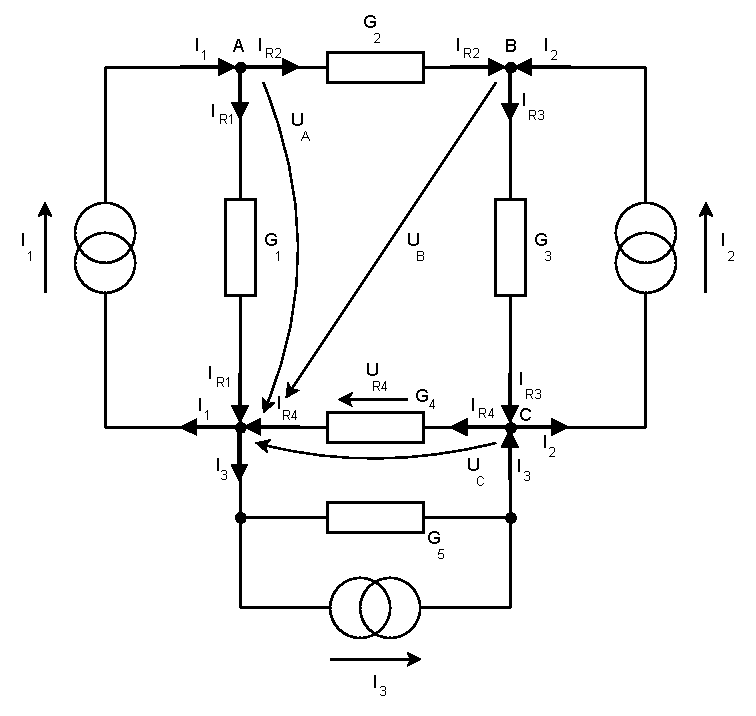
\includegraphics[scale=0.8,keepaspectratio]{xbednar00/zdroje/pr3/pr3_krok1.pdf}
\end{minipage}
\begin{minipage}{0.5\linewidth}
    $$I_3=\frac{U}{R_5}=3,75A$$\\
    $$G_1=\frac{1}{R_1}=\frac{1}{53}S$$
    $$G_2=\frac{1}{R_2}=\frac{1}{49}S$$
    $$G_3=\frac{1}{R_3}=\frac{1}{65}S$$ 
    $$G_4=\frac{1}{R_4}=\frac{1}{39}S$$
    $$G_5=\frac{1}{R_5}=\frac{1}{32}S$$
\end{minipage}
\end{figure}

\newpage
\subsection*{2. krok}
Vytvoríme rovnice napätia pre jednotlivé uzly.\\
    $$A:U_A(G_1+G_2)+U_B(-G_2)+U_C(0)-I_1=0$$
    $$B:U_A(-G_2)+U_B(G_2+G_3)+U_C(-G_3)-I_2=0$$
    $$C:U_A(0)+U_B(-G_3)+U_C(G_3+G_4+G_5)+I_2-I_3=0$$\\
Rovnice prevedieme na maticový tvar.\\
$$\begin{pmatrix}
    G_1+G_2 & -G_2 & 0\\
    -G_2 & G_2+G_3 & -G_3\\
    0 & -G_3 & G_3+G_4+G_5\\
\end{pmatrix}
\times
\begin{pmatrix}
    U_A\\
    U_B\\
    U_C\\
\end{pmatrix}
=
\begin{pmatrix}
    I_1\\
    I_2\\
    -I_2+I_3
\end{pmatrix}$$\\
Vyriešime pomocou Sarrusovho a Cramerovho pravidla a dostaneme výsledné napätia:\\
$$U_A=65,9954V\qquad U_B=82,9100V\qquad U_C \doteq 59,8478V$$\\
Na záver si vyjadríme $\pmb{U_{R_4}}$ a dopočítame $\pmb{I_{R_4}}$.\\
$$\pmb{U_{R_4}}=U_C \doteq \pmb{59,8478V}\qquad\qquad \pmb{I_{R_4}}=\frac{U_{R_4}}{R_4} \doteq \pmb{1,5346A}$$

    

